
\chapter{Numerical and Physical Accuracy\label{chpt:accuracy}}

This chapter gives a systematic comparison between algorithms for
the evaluation of the excess free energy $\mathcal{F}_{\mathrm{exc}}$
and its gradient $\gamma$ in terms of accuracy. As the theory does
not contain any unpredictable random part, the comportment of the
code is mathematically predictable. For example, certain algorithms
should give the same result at machine precision ($10^{-13}$ to $10^{-15}$)
in certain conditions. A lost of accuracy comparing to the prediction
can be classified as two different kinds. One is the theoretical lost,
for example, certain equation is only valid for an infinite order.
This kind of lost is unavoidable but should be worked out explicitly.
Another source is the unknown lost, contains all kinds of incompatibility
in the result that cannot explained mathematically. This kind of lost
can mainly due to a bug in the implementation that cannot be find
out, or it is a theoretical lost that haven't been worked out. They
also deserve a discussion. All those comparisons aim to give a global
view of the credibility of the results given by this code.

\section{Generalized spherical harmonics transform\label{sec:gsh-imp}}

As discussed in $\mathsection$\ref{sec:fgsht}, the function after
a forward-backward \acs{GSHT} process 
\begin{equation}
F_{\mu'\mu}^{m}=\frac{f_{m}}{8\pi^{2}}\sum_{i=0}^{m_{\mathrm{max}}}w_{i}\sum_{j=0}^{2m_{\mathrm{max}}}\sum_{k=0}^{2\left\lfloor m_{\mathrm{max}}/s\right\rfloor }F(\Theta_{i},\Phi_{j},\Psi_{k})R_{\mu'\mu}^{m*}(\Theta_{i},\Phi_{j},\Psi_{k})
\end{equation}
\begin{equation}
F(\Theta_{i},\Phi_{j},\Psi_{k})=\sum_{m=0}^{n_{\mathrm{max}}}f_{m}\sum_{\mu'=-m}^{m}\sum_{\underset{\mod(\mu,s)=0}{\mu=-m}}^{m}F_{\mu'\mu}^{m}R_{\mu'\mu}^{m}(\Theta_{i},\Phi_{j},\Psi_{k})
\end{equation}
only remains the same when it is a polynomial of both $\cos\Theta$,
$\cos\Phi$ and $\cos\Psi$ of order $n_{\max}$, where $n_{\max}$
is the highest order of \acs{GSH} in the expansion, and $m_{\max}=n_{\max}$
the order of quadrature used. However, as in the reality, the density
variable $\rho$ is not a simple polynomial, and the choice of $m_{\max}$
and $n_{\max}$ is tightly linked to the performance, it is important
to know how much these choices will affect the results. The \acs{FFT}
process is implemented by package FFTW3 \citep{FFTW3}, which is verified
to be leading to strictly no accuracy lost (at machine precision).
That means the \acs{FGSHT} process will have strictly with the \acs{GSHT}
process. Here we do not need to distinguish the two.

\subsection{$m_{\mathrm{max}}$ and $n_{\mathrm{max}}$ of projections}

The numerical error tests of a forward-backward GSHT process with
different order $n_{\mathrm{max}}$ of GSH and $m_{\mathrm{max}}$
of quadrature are shown in table \ref{tab:error-gsh}.
\begin{table}[H]
\begin{centering}
\subfloat[$f(\mathbf{\Omega})=1$]{\begin{centering}
\begin{tabular*}{1\columnwidth}{@{\extracolsep{\fill}}ccccccc}
\toprule 
{\footnotesize{}$m$\textbackslash{}$n$} & \multirow{1}{*}{{\footnotesize{}0}} & \multirow{1}{*}{{\footnotesize{}1}} & {\footnotesize{}2} & \multirow{1}{*}{{\footnotesize{}3}} & \multirow{1}{*}{{\footnotesize{}4}} & \multirow{1}{*}{{\footnotesize{}5}}\tabularnewline
\midrule
\multicolumn{1}{c}{{\footnotesize{}0}} & \textbf{\footnotesize{}0 (0)} & {\footnotesize{}9.00 (3.00)} & {\footnotesize{}34.00 (18.00)} & {\footnotesize{}83.00 (39.00)} & {\footnotesize{}164.00 (84.00)} & {\footnotesize{}285.00 (139.00)}\tabularnewline
\multicolumn{1}{c}{{\footnotesize{}1}} & \textbf{\footnotesize{}0 (0)} & \textbf{\footnotesize{}0 (0)} & {\footnotesize{}0 (1.67)} & {\footnotesize{}4.34 (6.07)} & {\footnotesize{}7.06 (13.63)} & {\footnotesize{}14.88 (17.30)}\tabularnewline
\multicolumn{1}{c}{{\footnotesize{}2}} & \textbf{\footnotesize{}0 (0)} & \textbf{\footnotesize{}0 (0)} & \textbf{\footnotesize{}0 (0)} & {\footnotesize{}0 (0)} & {\footnotesize{}0 (0)} & {\footnotesize{}5.65 (2.71)}\tabularnewline
{\footnotesize{}3} & \textbf{\footnotesize{}0 (0)} & \textbf{\footnotesize{}0 (0)} & \textbf{\footnotesize{}0 (0)} & \textbf{\footnotesize{}0 (0)} & {\footnotesize{}0 (0)} & {\footnotesize{}0 (0)}\tabularnewline
\multicolumn{1}{c}{{\footnotesize{}4}} & \textbf{\footnotesize{}0 (0)} & \textbf{\footnotesize{}0 (0)} & \textbf{\footnotesize{}0 (0)} & \textbf{\footnotesize{}0 (0)} & \textbf{\footnotesize{}0 (0)} & {\footnotesize{}0 (0)}\tabularnewline
\multicolumn{1}{c}{{\footnotesize{}5}} & \textbf{\footnotesize{}0 (0)} & \textbf{\footnotesize{}0 (0)} & \textbf{\footnotesize{}0 (0)} & \textbf{\footnotesize{}0 (0)} & \textbf{\footnotesize{}0 (0)} & \textbf{\footnotesize{}0 (0)}\tabularnewline
\bottomrule
\end{tabular*}
\par\end{centering}
}
\par\end{centering}
\begin{centering}
\subfloat[$f(\mathbf{\Omega})=\cos3\Theta$]{\begin{centering}
\begin{tabular*}{1\columnwidth}{@{\extracolsep{\fill}}ccccccc}
\toprule 
{\footnotesize{}$m$\textbackslash{}$n$} & \multirow{1}{*}{{\footnotesize{}0}} & \multirow{1}{*}{{\footnotesize{}1}} & {\footnotesize{}2} & \multirow{1}{*}{{\footnotesize{}3}} & \multirow{1}{*}{{\footnotesize{}4}} & \multirow{1}{*}{{\footnotesize{}5}}\tabularnewline
\midrule
\multicolumn{1}{c}{{\footnotesize{}0}} & {\footnotesize{}0 (0)} & {\footnotesize{}0 (0)} & {\footnotesize{}0 (0)} & {\footnotesize{}0 (0)} & {\footnotesize{}0 (0)} & {\footnotesize{}0 (0)}\tabularnewline
\multicolumn{1}{c}{{\footnotesize{}1}} & {\footnotesize{}0.96 (0.96)} & {\footnotesize{}0 (0)} & {\footnotesize{}0 (0)} & {\footnotesize{}2.56 (6.99)} & {\footnotesize{}10.76 (14.15)} & {\footnotesize{}13.83 (21.21)}\tabularnewline
\multicolumn{1}{c}{{\footnotesize{}2}} & {\footnotesize{}0.46 (0.46)} & {\footnotesize{}0 (0)} & {\footnotesize{}0 (0)} & {\footnotesize{}0 (0)} & {\footnotesize{}0 (0)} & {\footnotesize{}1.36 (0.50)}\tabularnewline
{\footnotesize{}3} & {\footnotesize{}0.86 (0.86)} & {\footnotesize{}0.66 (0.66)} & {\footnotesize{}0.66 (0.66)} & \textbf{\footnotesize{}0 (0)} & {\footnotesize{}0 (0)} & {\footnotesize{}0.66 (0.66)}\tabularnewline
\multicolumn{1}{c}{{\footnotesize{}4}} & {\footnotesize{}0.99 (0.99)} & {\footnotesize{}0.80 (0.80)} & {\footnotesize{}0.80 (0.80)} & \textbf{\footnotesize{}0 (0)} & \textbf{\footnotesize{}0 (0)} & {\footnotesize{}0 (0)}\tabularnewline
\multicolumn{1}{c}{{\footnotesize{}5}} & {\footnotesize{}0.83 (0.83)} & {\footnotesize{}1.01 (1.01)} & {\footnotesize{}1.01 (1.01)} & \textbf{\footnotesize{}0 (0)} & \textbf{\footnotesize{}0 (0)} & \textbf{\footnotesize{}0 (0)}\tabularnewline
\bottomrule
\end{tabular*}
\par\end{centering}
}
\par\end{centering}
\begin{centering}
\subfloat[$f(\mathbf{\Omega})=\cos3\Phi$]{\begin{centering}
\begin{tabular*}{1\columnwidth}{@{\extracolsep{\fill}}ccccccc}
\toprule 
{\footnotesize{}$m$\textbackslash{}$n$} & \multirow{1}{*}{{\footnotesize{}0}} & \multirow{1}{*}{{\footnotesize{}1}} & {\footnotesize{}2} & \multirow{1}{*}{{\footnotesize{}3}} & \multirow{1}{*}{{\footnotesize{}4}} & \multirow{1}{*}{{\footnotesize{}5}}\tabularnewline
\midrule
\multicolumn{1}{c}{{\footnotesize{}0}} & {\footnotesize{}0 (0)} & {\footnotesize{}9.00 (3.00)} & {\footnotesize{}34.00 (18.00)} & {\footnotesize{}83.00 (39.00)} & {\footnotesize{}164.00 (84.00)} & {\footnotesize{}285.00 (139.00)}\tabularnewline
\multicolumn{1}{c}{{\footnotesize{}1}} & {\footnotesize{}0 (0)} & {\footnotesize{}0 (0)} & {\footnotesize{}0 (1.67)} & {\footnotesize{}4.34 (6.07)} & {\footnotesize{}7.06 (13.63)} & {\footnotesize{}14.88 (17.30)}\tabularnewline
\multicolumn{1}{c}{{\footnotesize{}2}} & {\footnotesize{}1.00 (1.00)} & {\footnotesize{}1.00 (1.00)} & {\footnotesize{}0.50 (0.50)} & {\footnotesize{}1.53 (1.53)} & {\footnotesize{}1.15 (1.15)} & {\footnotesize{}3.65 (0.89)}\tabularnewline
{\footnotesize{}3} & {\footnotesize{}1.00 (1.00)} & {\footnotesize{}1.00 (1.00)} & {\footnotesize{}1.00 (1.00)} & {\footnotesize{}0.83 (0.83)} & {\footnotesize{}1.10 (1.10)} & {\footnotesize{}1.11 (1.11)}\tabularnewline
\multicolumn{1}{c}{{\footnotesize{}4}} & {\footnotesize{}1.00 (1.00)} & {\footnotesize{}1.00 (1.00)} & {\footnotesize{}1.00 (1.00)} & {\footnotesize{}0.90 (0.90)} & {\footnotesize{}0.90 (0.90)} & {\footnotesize{}0.69 (0.69)}\tabularnewline
\multicolumn{1}{c}{{\footnotesize{}5}} & {\footnotesize{}1.00 (1.00)} & {\footnotesize{}1.00 (1.00)} & {\footnotesize{}1.00 (1.00)} & {\footnotesize{}0.94 (0.94)} & {\footnotesize{}0.94 (0.94)} & {\footnotesize{}0.80 (0.80)}\tabularnewline
\bottomrule
\end{tabular*}
\par\end{centering}
}
\par\end{centering}
\begin{centering}
\subfloat[$f(\mathbf{\Omega})=R_{30}^{3}(\mathbf{\Omega})$]{\begin{centering}
\begin{tabular*}{1\columnwidth}{@{\extracolsep{\fill}}ccccccc}
\toprule 
{\footnotesize{}$m$\textbackslash{}$n$} & \multirow{1}{*}{{\footnotesize{}0}} & \multirow{1}{*}{{\footnotesize{}1}} & {\footnotesize{}2} & \multirow{1}{*}{{\footnotesize{}3}} & \multirow{1}{*}{{\footnotesize{}4}} & \multirow{1}{*}{{\footnotesize{}5}}\tabularnewline
\midrule
\multicolumn{1}{c}{{\footnotesize{}0}} & {\footnotesize{}0 (0)} & {\footnotesize{}5.03 (1.68)} & {\footnotesize{}19.01 (10.06)} & {\footnotesize{}46.40 (21.80)} & {\footnotesize{}91.68 (46.96)} & {\footnotesize{}- (77.70)}\tabularnewline
\multicolumn{1}{c}{{\footnotesize{}1}} & {\footnotesize{}0 (0)} & {\footnotesize{}0 (0)} & {\footnotesize{}0 (0.51)} & {\footnotesize{}1.32 (1.85)} & {\footnotesize{}2.15 (4.15)} & {\footnotesize{}4.53 (5.26)}\tabularnewline
\multicolumn{1}{c}{{\footnotesize{}2}} & {\footnotesize{}0.56 (0.56)} & {\footnotesize{}0.56 (0.56)} & {\footnotesize{}0.07 (0.07)} & {\footnotesize{}0.55 (0.55)} & {\footnotesize{}0.76 (0.76)} & {\footnotesize{}2.05 (1.00)}\tabularnewline
{\footnotesize{}3} & {\footnotesize{}0.47 (0.47)} & {\footnotesize{}0.47 (0.47)} & {\footnotesize{}0.47 (0.47)} & \textbf{\footnotesize{}0 (0)} & {\footnotesize{}0.46 (0.46)} & {\footnotesize{}0.46 (0.46)}\tabularnewline
\multicolumn{1}{c}{{\footnotesize{}4}} & {\footnotesize{}0.56 (0.56)} & {\footnotesize{}0.56 (0.56)} & {\footnotesize{}0.56 (0.56)} & \textbf{\footnotesize{}0 (0)} & \textbf{\footnotesize{}0 (0)} & {\footnotesize{}0 (0)}\tabularnewline
\multicolumn{1}{c}{{\footnotesize{}5}} & {\footnotesize{}0.51 (0.51)} & {\footnotesize{}0.51 (0.51)} & {\footnotesize{}0.51 (0.51)} & \textbf{\footnotesize{}0 (0)} & \textbf{\footnotesize{}0 (0)} & \textbf{\footnotesize{}0 (0)}\tabularnewline
\bottomrule
\end{tabular*}
\par\end{centering}
}
\par\end{centering}
\caption[Maximum absolute error $E_{a}^{\mathrm{max}}$ introduced by a forward-backward
GSHT process]{Maximum absolute error $E_{a}^{\mathrm{max}}$ introduced by a forward-backward
GSHT process of function $f$ (outside the parentheses) and the corresponding
transform for function with $\mathrm{C}_{2v}$ symmetry (with two
times less $\Psi$ points of quadrature, inside the parentheses).
Differences should be theoretically null in the table is in bold character.
\label{tab:error-gsh}}
\end{table}

It conforms the theoretical prediction where should lead to no accuracy
lost ($m_{\max}>n_{\max}$ and $f$ the polynomial that can be expanded
on \acs{GSH}s of order at most $n_{\max}$). It should be noted,
that as we do firstly a forward then a backward transform, when $m_{\max}<n_{\max}$,
even the input function is of order at most $m_{\max}$, the output
function is of order $n_{\mathrm{max}}$ in the presence of $R_{\mu'\mu}^{m}$
which is of order $n_{\mathrm{max}}$, thus the two functions are
different. The function in which the order of $\cos\Phi$ and $\cos\Psi$
is greater than $\cos\Theta$ (case of $f(\mathbf{\Omega})=\cos3\Phi$),
the two functions are different too, because it cannot be expanded
to a finite number of \acs{GSH}s.

\subsection{From $\rho$ to $\gamma$}

To conclude from above, the error for an arbitrary function like $\rho$,
which is not a combination of \acs{GSH}s, can be huge. One evidence
is the appearance of unphysical density $\rho(\mathbf{r},\mathbf{\Omega})<0$
at certain point after a forward-backward \acs{GSHT} process (figure
\ref{fig:unphysical-rho}). \textcolor{red}{(other better way?)}

\begin{figure}[h]
\begin{centering}
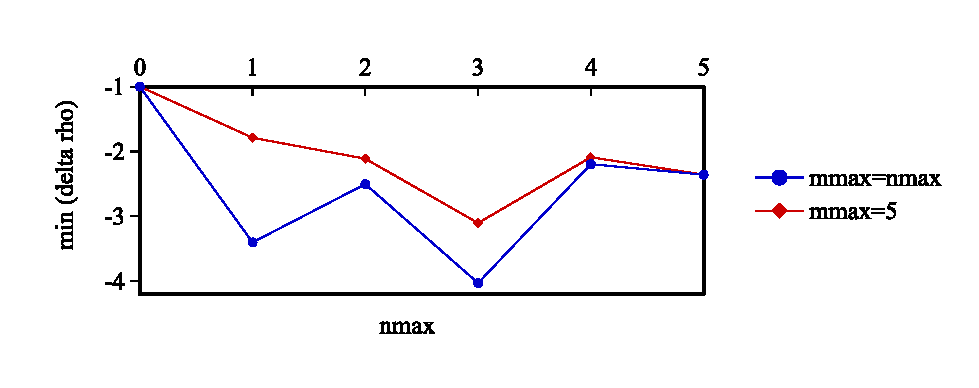
\includegraphics[bb=0bp 10bp 454bp 160bp,width=0.75\columnwidth]{_figure/results/min_delta_rho}
\par\end{centering}
\caption[The minimum value of $\Delta\rho(\mathbf{r},\mathbf{\Omega})/\rho_{0}$
after a forward-backward \acs{GSHT} process]{The minimum value of $\Delta\rho(\mathbf{r},\mathbf{\Omega})/\rho_{0}$
after a forward-backward \acs{GSHT} process with respect to $n_{\max}$.
Computed for a $45^{3}$ grid ($L=25$) for a converged density of
an artificial charged LJ center $\mathrm{CH}_{4}^{+0.4}$. \label{fig:unphysical-rho} }
\end{figure}

Theoretically, we expect this minimum value approach to zero when
increasing $m_{\max}$ or $n_{\max}$, which is not exactly the case.
That means perhaps the order of expansion is still far from to find
a tendency. Knowing that $\rho(\mathbf{r},\mathbf{\Omega})/\rho_{0}\rightarrow1$
far from the solute, the error can be said oblivious within the computing
capacity ($n_{\max}<5$), that means we cannot expand rightly the
density $\rho$ on \acs{GSH} projections, where. But this have a
much less effect on the functional gradient $\gamma$ that we evaluate,
because in a convolution product, $\Delta\hat{\rho}(\mathbf{k},\mathbf{\Omega})$
and the \acs{DCF} $\hat{c}(k,\mathbf{\Omega}_{1},\mathbf{\Omega}_{2})$
can be both expended, and product of higher order terms vanishes more
easily. Latter we will show that the profile of $\gamma$ and the
free energy $\mathcal{F}_{\mathrm{exc}}$ can already converge within
$n_{\max}<5$.

\section{Comparison between branches}

As shown in figure \ref{fig:Possible-algorithms}, if we fixe $\Delta\rho(\mathbf{r},\mathbf{\Omega})$
to a recombination of \acs{GSH} projections, all methods using the
same \acs{DCF} should give mathematically identical results. The
most direct comparison is the free energy evaluated during 1 iteration.
And to be more strict, is also interesting to compare the profile
of $\gamma$.

\subsection{Difference in energy evaluation}

As shown in table \ref{tab:free-energy}, the methods using the same
\acs{DCF} at the same $m_{\max}$ which is mathematically identical
in an infinite condition, give nearly the same results.

\begin{table}[H]
\begin{centering}
\begin{tabular*}{1\linewidth}{@{\extracolsep{\fill}}llll}
\toprule 
\tableheadline{Method} & $n_{\max}$ & \tableheadline{DCF} & \tableheadline{Free Energy} {\footnotesize{}(kJ/mol)}\tabularnewline
\midrule
\texttt{\textbf{\footnotesize{}dipole}} & {\footnotesize{}1} & {\footnotesize{}{[}ref mdft{]}} & {\footnotesize{}13.1915264499904339}\tabularnewline
\texttt{\textbf{\footnotesize{}naive\_dipole}} & {\footnotesize{}1} & {\footnotesize{}{[}ref mdft{]}} & {\footnotesize{}13.1915269013357985}\tabularnewline
\midrule 
\texttt{\textbf{\footnotesize{}naive\_nmax1}} & {\footnotesize{}1} & {\footnotesize{}{[}ref Luc{]}{*}} & {\footnotesize{}18.6052247636086854}\tabularnewline
\texttt{\textbf{\footnotesize{}convolution\_standard}} & {\footnotesize{}1} & {\footnotesize{}{[}ref Luc{]}{*}} & {\footnotesize{}18.6093390102806886}\tabularnewline
\midrule 
\texttt{\textbf{\footnotesize{}naive\_interpolation}} & {\footnotesize{}2} & {\footnotesize{}{[}ref Luc{]}} & {\footnotesize{}26.8444355457069044}\tabularnewline
\texttt{\textbf{\footnotesize{}naive\_standard}} & {\footnotesize{}2} & {\footnotesize{}{[}ref Luc{]}} & {\footnotesize{}26.9897310488084479}\tabularnewline
\texttt{\textbf{\footnotesize{}convolution\_standard}} & {\footnotesize{}2} & {\footnotesize{}{[}ref Luc{]}} & {\footnotesize{}26.9163932581793155}\tabularnewline
\texttt{\textbf{\footnotesize{}convolution\_asymm}} & {\footnotesize{}2} & {\footnotesize{}{[}ref Luc{]}} & {\footnotesize{}26.9163932581793155}\tabularnewline
\texttt{\textbf{\footnotesize{}convolution\_pure\_angular}} & {\footnotesize{}2} & {\footnotesize{}{[}ref Luc{]}} & {\footnotesize{}26.9163932581793155}\tabularnewline
\bottomrule
\end{tabular*}
\par\end{centering}
\caption[Free energy calculated during 1 iteration]{Free energy calculated during 1 iteration for a $32^{3}$ grid ($L=20\textrm{Å}$)
for a fake LJ center $\mathrm{CH_{4}^{+0.33}}$, using a converged
density as input. Here $m_{\max}=n_{\max}$. \textcolor{red}{``{*}''
means without correction.}\label{tab:free-energy}}
\end{table}
 

The light difference between \texttt{\textbf{naive\_nmax1}} and \texttt{\textbf{convolution\_standard}}
at $m_{\max}=1$ is due to the artificial decoration at $k$-border
showing in later section, and the difference between \texttt{\textbf{naive\_interpolation}}
and \texttt{\textbf{naive\_standard}} and \texttt{\textbf{convolution}}
methods are also acceptable, which is natural to be lightly different
due to the interpolation error and the \acs{GSH} expansion (the $\rho$
recombination of \acs{GSH} projections will be discussed later).
This supports by the way that we do not need the same order of \acs{GSH}
expansion for $\gamma$ than for $\Delta\rho$.

\subsection{A single k-kernel\label{subsec:A-single-k-kernel}}

Firstly, we are interested in the local paths from $\Delta\hat{\rho}_{\mu'\mu}^{m}(\mathbf{k})$
to $\hat{\gamma}_{\mu'\mu}^{m}(\mathbf{k})$ , that can be tested
independently for a certain $\mathbf{k}$. As shown in figure \ref{fig:k-kernel},
four algorithms are available to the purpose.

\begin{figure}[h]
\begin{centering}
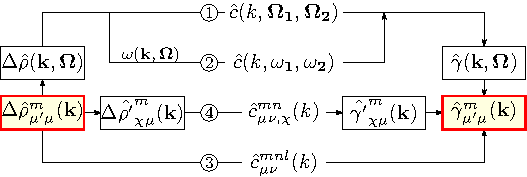
\includegraphics{_figure/algorithms_q}
\par\end{centering}
\caption{Schema of a k-kernel test \label{fig:k-kernel} }
\end{figure}

The program that compares each element of $\hat{\gamma}_{\mu'\mu}^{m}(\mathbf{k})$
issued from these 4 algorithms for a given $\Delta\hat{\rho}_{\mu'\mu}^{m}(\mathbf{k})$
is done by Mr. Luc Belloni, which shows that the $\hat{\gamma}_{\mu'\mu}^{m}(\mathbf{k})$
for the four algorithms are strictly identical. This means, the final
result of energy and structure is independent to the choice of path
inside a $k$-kernel, if $\Delta\hat{\rho}(\mathbf{k},\mathbf{\Omega})$
can be fully expended on \acs{GSH}s.

\subsection{k-border effect\label{subsec:k-border-effect}}

Here we test the whole process shown in figure \ref{fig:Possible-algorithms},
with $\Delta\rho(\mathbf{r},\mathbf{\Omega})$ generated from a recombination
of \acs{GSH} projections. Firstly, we compare the three \texttt{\textbf{convolution}}
algorithms passing by \acs{GSH} expansion. For a $64^{3}$ grid,
$n_{\max}=3$, the three algorithms \texttt{\textbf{convolution\_standard}},
\texttt{\textbf{convolution\_asymm}}, and \texttt{\textbf{convolution\_pure\_angular}}
gives the same free energy, but lightly different result when comparing
each element of $\gamma(\mathbf{r},\mathbf{\Omega})$, and this difference
seems to decrease when increase the number of grid points. More, the
projections $\gamma_{\mu'\mu}^{m}(\mathbf{r})$ which should be purely
real as explained in $\mathsection$\ref{subsec:Reduction-by-symmetry},
have a light imaginary part. But surprisingly, for a $65^{3}$ grid,
it gives numerically the same result for both the three algorithms
at machine precision.{*} \marginpar{{*} The detailed value of $\gamma$ which the paragraph of description
is based on haven't been noted, as it was regarded as a bug in the
code at that time, and the code had been then modified; and to redo
such a process takes a lot of time.}

The difference between these methods is found to be a special $k$-border
effect linking to even number grids.

As the symmetry
\begin{equation}
\Delta\hat{\rho'}_{\chi\mu}^{m}(\mathbf{k})=(-)^{m+\mu+\chi}\Delta\hat{\rho'}_{\chi,-\mu}^{m*}(-\mathbf{k})\label{eq:2-1}
\end{equation}
 is generated by two symmetries

\begin{equation}
\Delta\hat{\rho}_{\mu'\mu}^{m}(\mathbf{k})=(-)^{\mu'+\mu}\Delta\hat{\rho}_{-\mu',-\mu}^{m*}(-\mathbf{k})\label{eq:1-1}
\end{equation}

\begin{equation}
R_{\mu'\chi}^{m}(\hat{k})=(-)^{m+\mu'+\chi}R_{-\mu',\chi}^{m}(-\hat{k})\label{eq:3-1}
\end{equation}

For the points ``at border'', it's to say that after the FFT where
the point having $\pm k_{i}=k_{i}^{\mathrm{max}}$, $i=1,2,3$, for
example for $k_{1},$

\[
\Delta\hat{\rho}_{\mu'\mu}^{m}(\pm k_{1},k_{2},k_{3})=\Delta\hat{\rho}_{\mu'\mu}^{m}(k_{1}^{\mathrm{max}},k_{2},k_{3})
\]
is naturally put in the same array by FFT for the grids having even
number,\marginpar{For example, for a grid 1D, the FFT having 6 points gives the values
for indices 0,1,2,3,-2,-1, and the FFT having 7 points gives the values
for 0,1,2,3,-3,-2,-1.} as shown in figure \ref{fig:k-border-effect}. 

\begin{figure}[h]
\begin{centering}
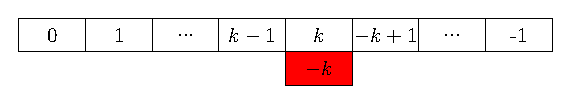
\includegraphics{_figure/k-border}
\par\end{centering}
\caption{$k$-border effect\label{fig:k-border-effect}}
\end{figure}

As \acs{FFT} possesses periodicity, the symmetry \ref{eq:1-1} can
always be respected at border. However, as

\begin{equation}
R_{-\mu',\chi}^{m}(-\hat{k}\equiv(-k_{1},-k_{2},-k_{3}))\neq R_{\mu',\chi}^{m}(k_{1}^{\mathrm{max}},-k_{2},-k_{3})
\end{equation}
the symmetries (\ref{eq:3-1}) and (\ref{eq:2-1}) are not respected
for these points. In the backward process, if we make sense of all
the $\gamma_{\mu'\mu}^{m}(\mathbf{k})$, as

\[
\gamma_{\mu'\mu}^{m}(-\hat{k}\equiv(-k_{1},-k_{2},-k_{3}))\neq\gamma_{\mu'\mu}^{m}(k_{1}^{\mathrm{max}},-k_{2},-k_{3})
\]
the symmetry

\begin{equation}
\gamma_{\mu'\mu}^{m}(\mathbf{k})=(-)^{\mu'+\mu}\gamma_{-\mu',-\mu}^{m*}(-\mathbf{k})\label{eq:1-1}
\end{equation}
is not respected totally, and this imposes that $\gamma_{\mu'\mu}^{m}(\mathbf{r})$
have a imaginary part. This imaginary part has been omitted implicitly
in the ``real to complex'' \acs{FFT} process of used in for example
\texttt{\textbf{convolution\_standard}}, for \acs{FGSHT}, or \texttt{\textbf{convolution\_pure\_angular}}
for FFT3D process. It is to say, we keep only the part of none-negative
$\mathbf{k}$ or none-negative $\mu$, supposing that the part we
omit respects the symmetry.

The right way to treat this issue is to artificially impose at the
border:
\begin{equation}
R_{\mu',\chi}^{m}(k_{i}^{\mathrm{max}})=\frac{1}{2}\left[R_{\mu',\chi}^{m}(k_{i})+R_{\mu',\chi}^{m}(-k_{i})\right]
\end{equation}
where $i$ is the conflict index in figure \ref{fig:k-border-effect}.
If more than one dimensions are in conflict, this process can be done
twice (4 terms for ``edges'' of the cube) or three times (8 terms
for ``vertices''). The point $\mathbf{k}=\hat{0}$ is different,
as it was define along $z$ axes to avoid implementation crash, it
doesn't respect eq. (\ref{eq:3-1}) and (\ref{eq:2-1}) neither. But
this point compared to hundreds thousands of total points is negligible.

The energies given by \texttt{\textbf{naive\_standard}} and the \texttt{\textbf{convolution}}
algorithms are identical for a $65^{3}$ and $n_{\max}=3$ grid, but
the element of $\gamma(\mathbf{r},\mathbf{\Omega})$ have a mysterious
difference at order of $10^{-2}$, seemed to be aleatory. A test redone
for a $45^{3}$ grid is shown in figure \ref{fig:Difference-in-gamma}.

\begin{figure}[H]
\begin{centering}
\subfloat[$\delta\hat{\gamma}(\mathbf{k},\mathbf{\Omega})$]{\begin{centering}
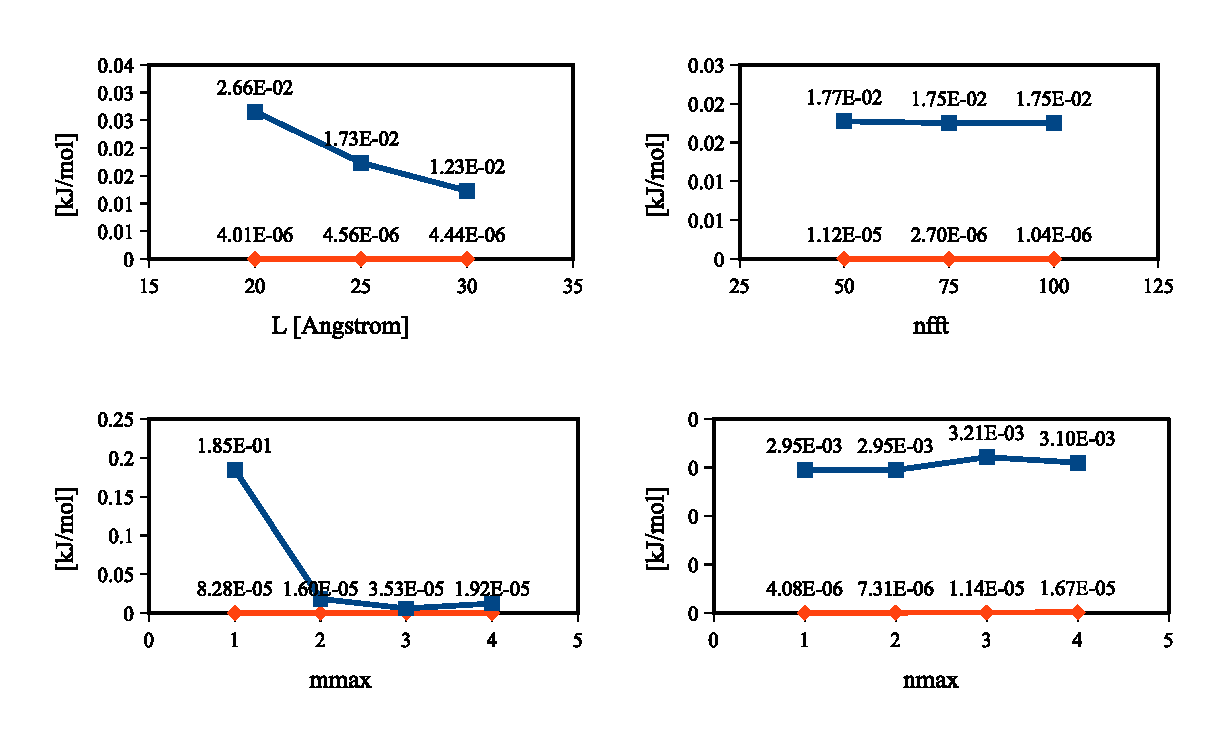
\includegraphics[width=0.75\columnwidth]{_figure/results/diff_k_gamma}
\par\end{centering}

}
\par\end{centering}
\begin{centering}
\subfloat[$\delta\gamma(\mathbf{r},\mathbf{\Omega})$]{\begin{centering}
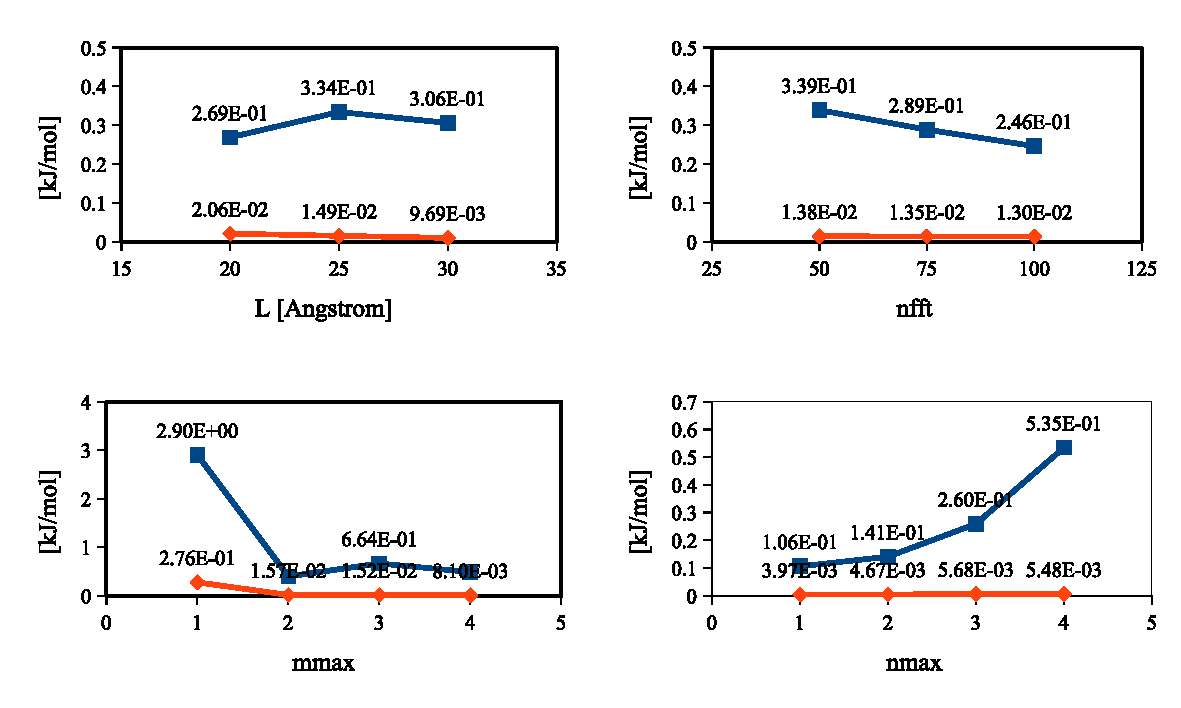
\includegraphics[width=0.75\columnwidth]{_figure/results/diff_gamma}
\par\end{centering}
}
\par\end{centering}
\caption[Maximum and average difference in $\hat{\gamma}(\mathbf{k},\mathbf{\Omega})$
and $\gamma(\mathbf{r},\mathbf{\Omega})$]{Maximum and average difference in $\hat{\gamma}(\mathbf{k},\mathbf{\Omega})$
and $\gamma(\mathbf{r},\mathbf{\Omega})$, for tests of different
box length$L$, different number of grid nfft in one dimension, $n_{\max}=1,4$
for $m_{\max}=n_{\max}$, and $n_{\max}=1,4$ for $m_{\max}=5$.\label{fig:Difference-in-gamma}}
\end{figure}

We can conclude very rudely that this error depends on the angular
quadrature $m_{\max}$. The dependence is natural, as the difference
between algorithms \texttt{\textbf{naive}} and \texttt{\textbf{convolution}}
is the treatment of the angular part. There is also a dependence on
$L$ in the $k$-space, but after \acs{FFT} it is mixed. The augmentation
of error in the $n_{\max}$ chart is unnatural, implying there is
perhaps a still bug in the code.

In a word, this mysterious difference cannot be yet explained, as
the \texttt{\textbf{naive}} methods does not have the $k$-border
effect linked to symmetry, on the other hand we used a odd grid, we
could not yet distinguish that it is a bug in the implementation,
in the test or in the theory. The projections $\gamma_{\mu\nu}^{mnl}(r)$
of this two algorithms seems to be identical (figure \ref{fig:gamma-proj}),
it is to say, the global structure of this two algorithms are almost
the same, and the error would not be very decisive.

\begin{figure}[h]
\begin{centering}
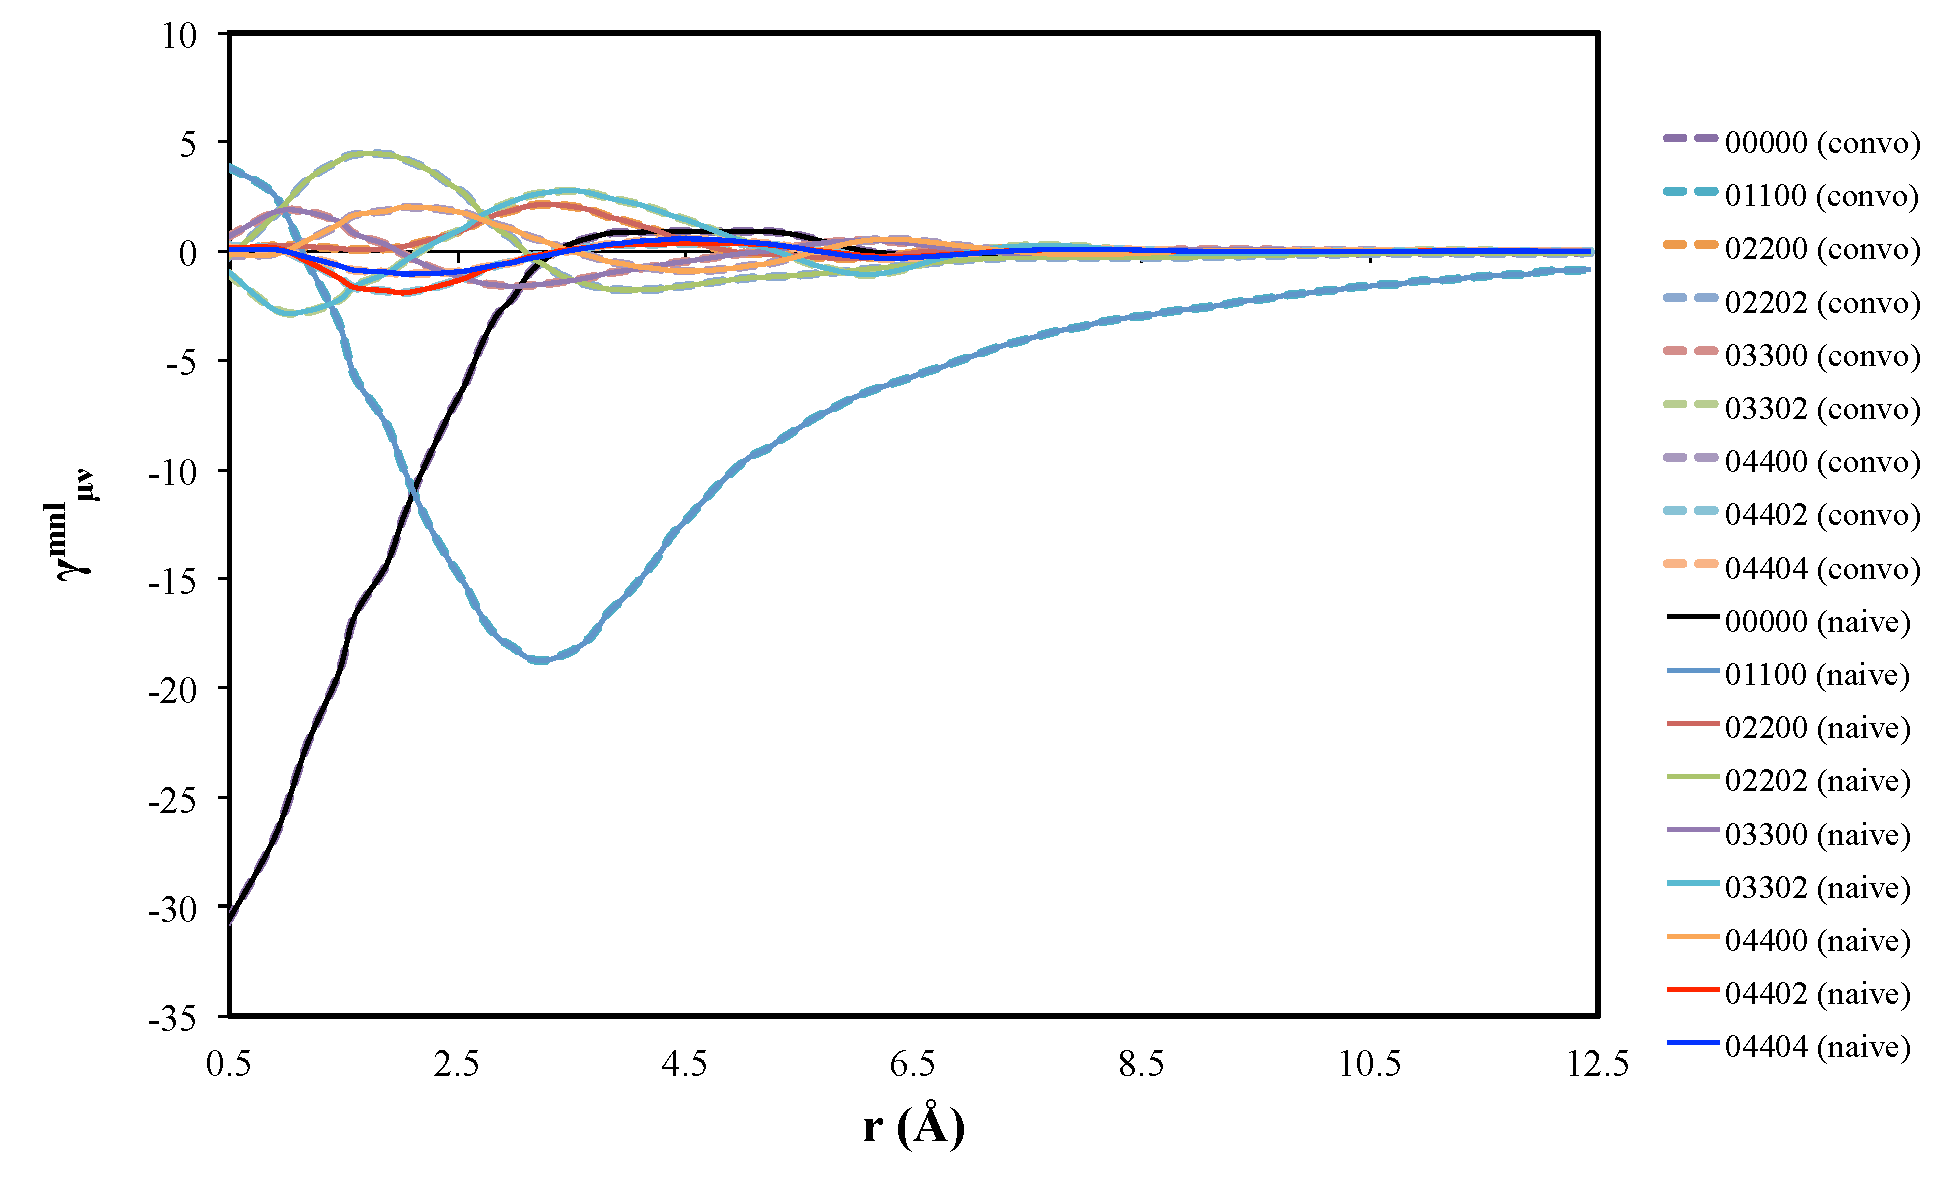
\includegraphics[width=0.65\columnwidth]{_figure/results/gamma_proj}
\par\end{centering}
\caption{A selection of rotational invariant projections $\gamma_{\mu\nu}^{mnl}(r)$
for a $65^{3}$ grid\label{fig:gamma-proj}}
\end{figure}


\section{Intrinsic variation of free energy}

Before study of free energy dependence on angular algorithms, we are
interested in the grid dependance, with can have an influence to the
tests later.

\begin{figure}[H]
\begin{centering}
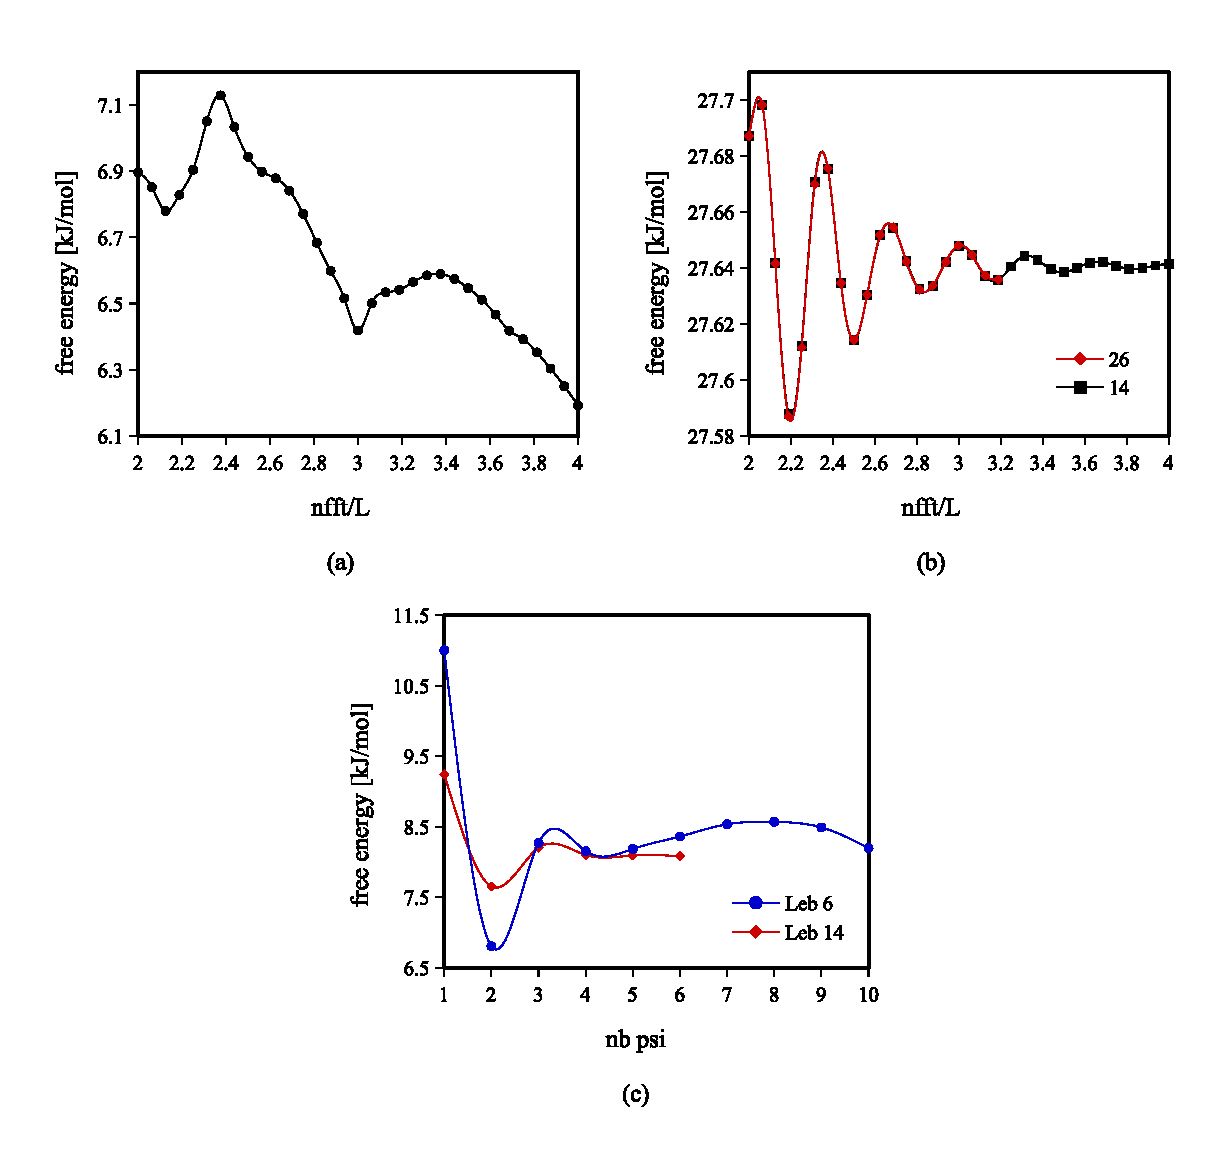
\includegraphics[width=0.75\columnwidth]{_figure/results/grid_reso}
\par\end{centering}
\caption[Space-grid and $\Psi$ dependence of code MDFT]{Space-grid and $\Psi$ dependence of code MDFT. $L=32$.(a) $\mathrm{CH_{4}^{+0.33}}$
using dipole DCF with $m_{\max}=1$; (b) $\mathrm{CH_{4}}$ using
DCF of $m_{\max}=5$, Lebedev quadrature of order 1 and 2; (c) acetone
using dipole DCF and Lebedev quadrature, varying $\Psi$, nfft=128.
\label{fig:Space-grid-and-psi-dependence}}
\end{figure}

As shown in figure \ref{fig:Space-grid-and-psi-dependence} (a) and
(b), there is a dependence of calculated free energy on the space
grid resolution. for a charged solute, the energy has tendency to
decrease when increasing the resolution of grid (nfft). And this decrease
does not link to the border correction mentioned in $\mathsection$...
, as the box length and the charge remain the same for the whole set
of test. From (b) we consider that at least 3 points grid in one dimension
per Angstrom is needed to reduce the uncertainty due to grid resolution.
Figure (c) fixed the Lebedev quadrature for $\Theta$ and $\Phi$,
but leaved varying the $\Psi$. We can also see a dependence on $\Psi$.
which does not vanish when increasing the resolution of grid. As during
the whole thesis the $\Psi$ is theoretically fixed in the same order
with $\Theta$ and $\Phi$, this remains an issue for further verification.
We can roughly conclude that an error around 1 kJ/mol is common for
this code.

\section{Series of charged LJ centre}

To valid the method, we chose a series of LJ centre, which possess
the LJ parameters of $\mathrm{C}\mathrm{H}_{4}$ in ref {[}{]}, and
have a various charge from -1.0 to 1.0 (table \ref{tab:Parameters-of-charged-met}).\marginpar{Here we use 298K according to habitude instead of 303K recommended
in reference \textcolor{red}{{[}ref{]}}, For both MDFT, IET, and DM
results.}

\begin{table}[h]
\begin{centering}
\begin{tabular*}{1\linewidth}{@{\extracolsep{\fill}}llllllll}
\toprule 
\tableheadline{Charge} & $\sigma$ {[}$\textrm{Å}${]} & $\epsilon$ {[}$\mathrm{kJ\cdot mol^{-1}}${]} & $x$ {[}$\textrm{\AA}${]} & $y$  {[}$\textrm{\AA}${]} & $z$ {[}$\textrm{\AA}${]} & $T$ {[}K{]} & \tableheadline{Number Density} {[}$\lyxmathsym{\AA}^{-3}${]}\tabularnewline
\midrule
-1.0 to 1.0 & 3.73  & 1.23  & 0 & 0 & 0 & 298 & 0.0332891\tabularnewline
\bottomrule
\end{tabular*}
\par\end{centering}
\caption{Parameters of charged Lenard-Jones centre (modified from $\mathrm{C}\mathrm{H}_{4}$)
\label{tab:Parameters-of-charged-met}}
\end{table}


\subsection{Box length dependance and charge dependance of free energy}

As discussed in section \ref{chpt:thermodynamic-quantities}, for
single ions, two types of corrections need to be added on the free
energy, which depend on the box length and and charge of the ion.
To verify these dependence, we implement a systematic calculation
from charge shown in figure

\begin{figure}[h]
\begin{centering}
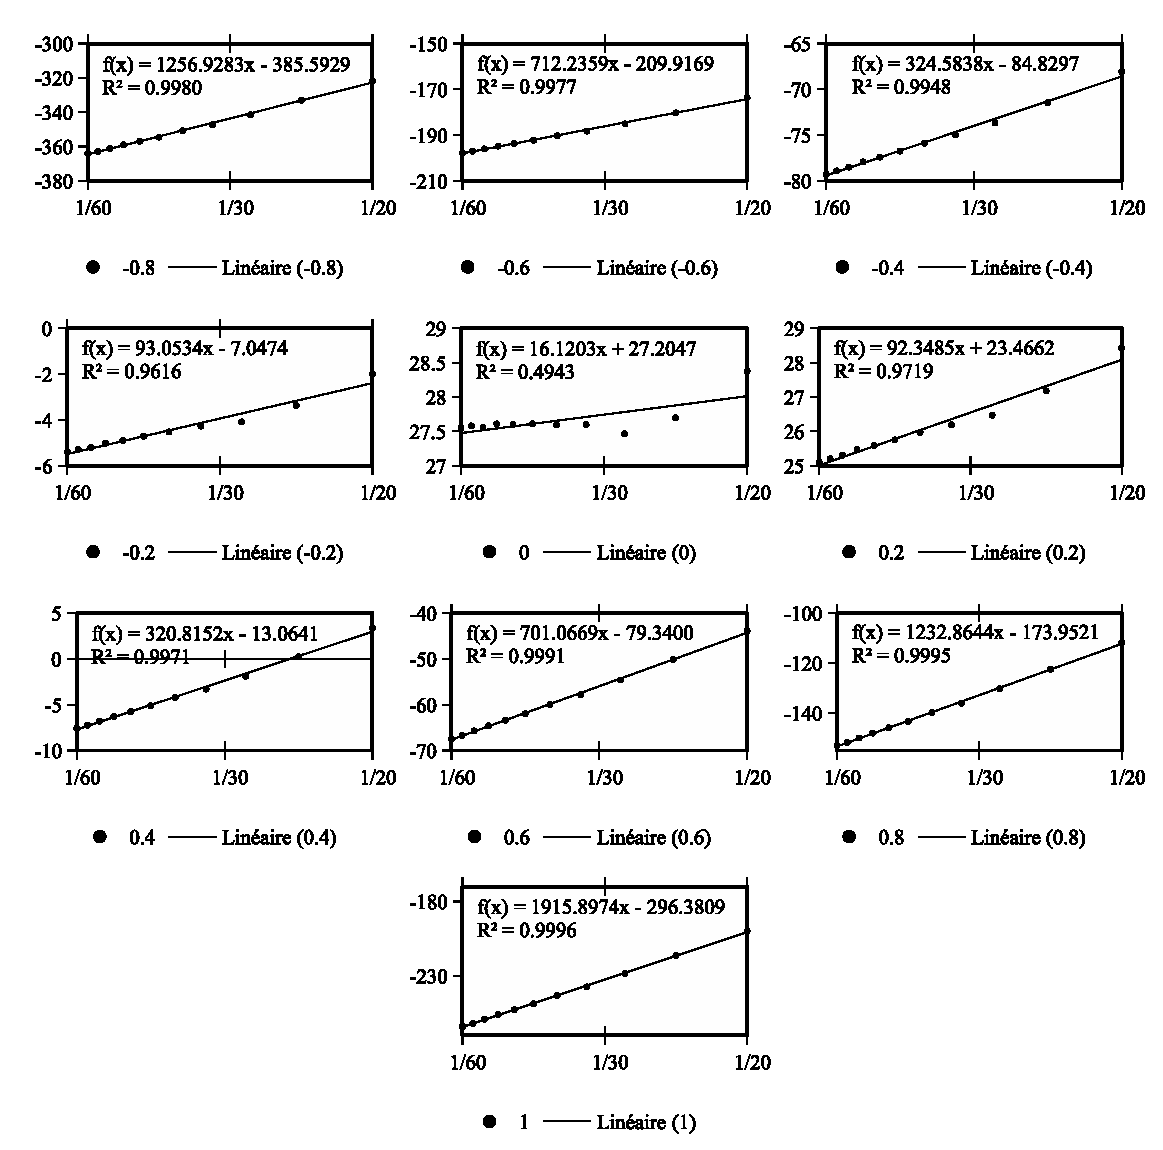
\includegraphics[width=1\columnwidth]{_figure/results/ch4_nmax1_lmn}
\par\end{centering}
\caption{free energy (without correction) of charged $\mathrm{C}\mathrm{H}_{4}$
centre (-1.0 to 1.0) with respect to the box length}
\end{figure}

\begin{figure}[h]
\begin{centering}
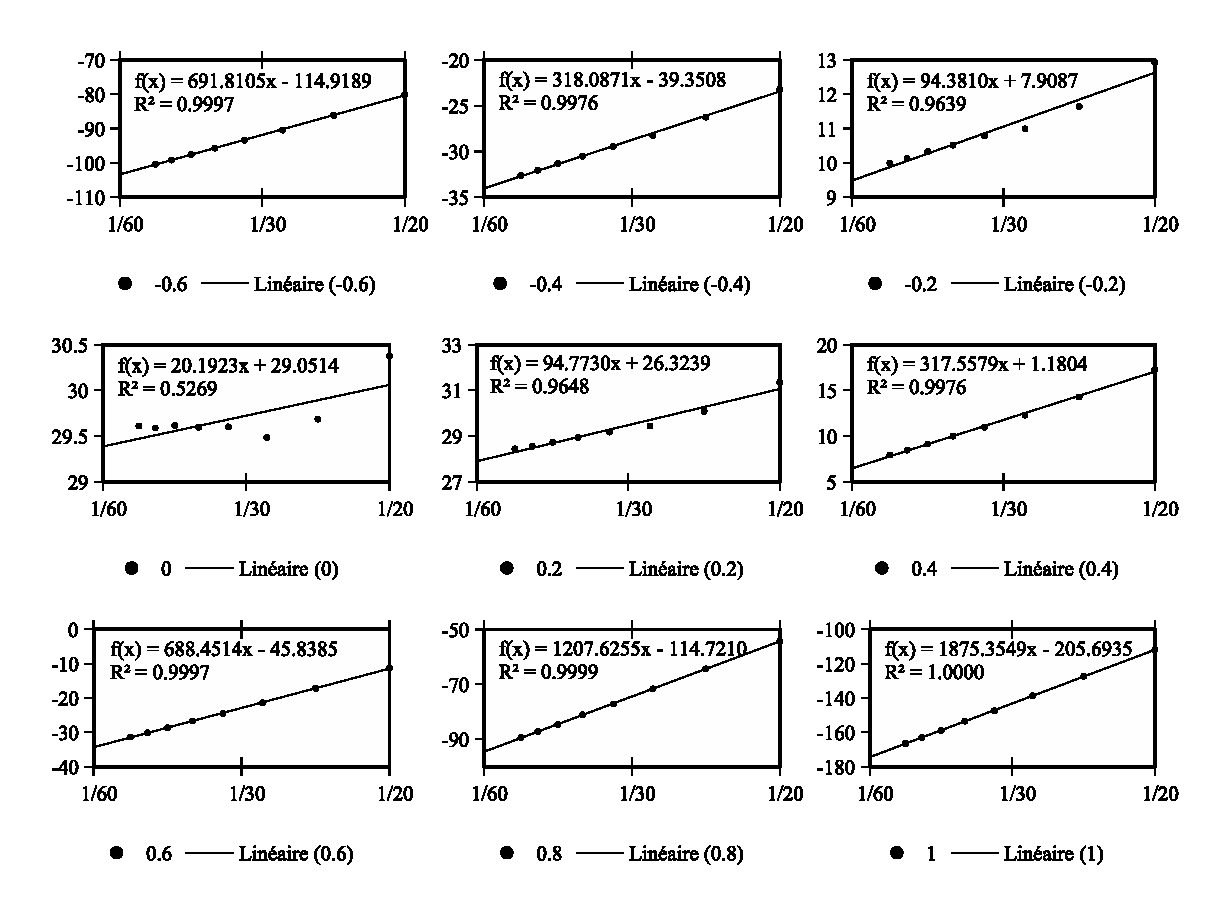
\includegraphics[width=1\columnwidth]{_figure/results/ch4_nmax5_inter}
\par\end{centering}
\caption{free energy (without correction) of charged $\mathrm{C}\mathrm{H}_{4}$
centre (-1.0 to 1.0) with respect to the box length}
\end{figure}

Continuum model correction at boundary

\begin{figure}[h]
\caption{Parabolic charge dependence of free energy of $\mathrm{C}\mathrm{H}_{4}$
centre series}
\end{figure}

It satisfies the Born model.

memory leak can cause divergence.

\subsection{Comparison with IET}

\begin{figure}[h]
\caption{Linear dependence of charge in the comparison to IET. Old algorithm
/ new algorithm, without correction}
\end{figure}

\begin{figure}[h]
\caption{Comparison to IET. Old algorithm / new algorithm, with P-scheme correction}
\end{figure}

Old data in appendix \ref{chpt:original_data}, which use 2m phi.
It gives quite similar result, which shows the insensibility of grid.

\subsection{Comparison with DM }

\section{Premier conclusion}

Capable to produce the same result with IEM, but have more ability
to calculate 3D molecules which is not suitable for spherical coordinates.

Interpolation is more stable compared to convolution and use less
angles compared to naive\_standard
